% !TEX root = ../main.tex
% !TEX program = xelatex

\chapter{ExRORU的实现与实验}\label{cha:experiment}

\section{ExRORU算法的实现}\label{sec:implementation}
本文实现的ExRORU算法基于jbpt\footnote{\url{https://code.google.com/p/jbpt}}中的CPU抽取WF-net的ExRORU关系并以矩阵形式展现,相关代码已开源共享在Github上\footnote{\url{https://github.com/shudiwsh2009/ExRORU}}。ExRORU算法的开发环境为IntelliJ IDEA 2016.1,JDK版本为1.8.0\_72。该算法接收一个PMNL文件为输入,将其解析为Petri网对象并抽取它所含的变迁之间的ExRORU关系,以矩阵形式输出。图\ref{fig:class_diagram}是该算法的类图。下面对该算法涉及到的主要类进行介绍。

\begin{figure}[htbp]
  \centering
  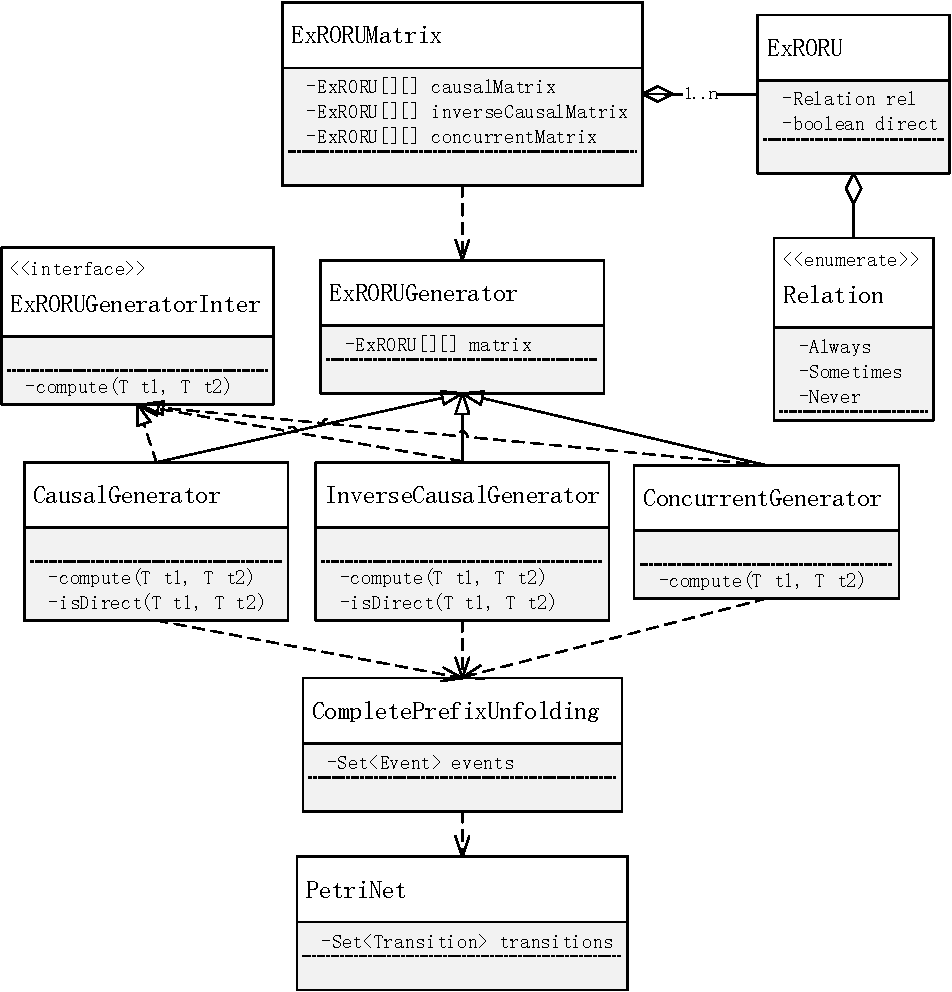
\includegraphics[width=0.9\textwidth]{class_diagram}
  \caption{ExRORU算法的实现类图}
  \label{fig:class_diagram}
\end{figure}

ExRORUMatrix是算法主类,主要功能是读入Petri网文件,并调用下层类抽取该Petri网的ExRORU矩阵。该类首先调用jbpt项目中的CPU计算方法构造给定Petri网对应的CPU,其后基于CPU抽取事件间ExRORU关系并依据前文算法折叠得到变迁间ExRORU关系。其中关键成员变量包括三个矩阵,分别对应变迁间的因果关系、逆因果关系和并行关系,每种关系都由ExRORU类记录。ExRORU类中包含标识不确定性的枚举型变量Relation和标记直接因果关系的布尔值变量(仅用于因果关系和逆因果关系)。

PetriNet类和CompletePrefixUnfolding类是jbpt项目中的原有类,分别存储Petri网和对应的完全前缀展开。在CPU的构造过程中,变迁与事件之间的对应关系也被记录下来用于后期的折叠过程。

ExRORUGenerator是抽取变迁间ExRORU关系的主类,其调用了三个不同的类分别抽取因果关系、逆因果关系和并行关系。这三个不同的类统一实现了ExRORUGeneratorInter接口,提供了compute(T t1, T t2)方法用于计算两个给定变迁之间的ExRORU关系,此外用于抽取因果关系和逆因果关系的CausalGenerator和InverseCausalGenerator还额外提供了isDirect(T t1, T t2)方法用于判定两个变迁是否满足定义\ref{def:exroru_event_causal_direct}中的直接和间接因果关系。三个类使用第\ref{cha:exroru}章介绍的算法首先基于CPU计算事件间的ExRORU关系然后将其折叠得到变迁间的ExRORU关系。

\section{实验设计与分析}\label{sec:experiment}
本节介绍ExRORU的实验设计与分析,主要包括有效性实验(将ExRORU与其他算法比较区分过程模型的能力)、性能实验(使用实际模型数据集衡量ExRORU算法的效率)和扩展性实验(衡量ExRORU处理含多并发结构过程模型的能力)等。

\subsection{有效性实验}\label{subsec:effectiveness}
本小节主要展示ExRORU算法强大的刻画过程模型行为语义的能力,并通过在多个模型实例中与第\ref{cha:related_work}章中介绍的算法对比,以说明其区分含有不同行为语义的过程模型的能力。

{\heiti 非自由选择结构\qquad}过程模型的任务之间存在间接依赖关系\cite{van2004workflow,van2003workflow,de2003workflow,van2004process},在WF-net上造成了非自由选择结构的存在(即选择关系与同步关系混合的情况)。图\ref{fig:nfc_example_1}中的模型是一个典型的含有非自由选择结构的模型,其中变迁$D$和变迁$E$之间存在非自由选择情形,即他们的执行并不由自身所决定,而是由之前被执行的变迁$A$和变迁$B$决定。具体分析,当在该WF-net的源库所$P_{0}$中放置一个托肯时,变迁$A$和变迁$B$同时被使能,若此时选择触发变迁$A$,则会在库所$_{1}$和库所$P_{2}$中各产生一个托肯;此时只有变迁$C$被使能,其被触发之后会消耗库所$P_{1}$的托肯,同时在库所$P_{4}$中产生一个托肯;库所$P_{2}$和库所$P_{4}$各有一个托肯时,显然只有变迁$D$被使能。另一方面,若一开始选择触发变迁$B$,同理可知在变迁$C$被触发之后只有变迁$E$被使能。因此,该模型的变迁执行序列只有$\langle A,C,D\rangle$和$\langle B,C,E\rangle$两条。

与之相对的是图\ref{fig:nfc_example_2}中不含有非自由选择结构的模型。与图\ref{fig:nfc_example_1}中的模型相比,该模型少了两个库所和四条边,其中变迁$D$和变迁$E$不存在非自由选择情形,即他们的执行由自身竞争库所$P_{2}$中的托肯所决定。因此,该模型的变迁执行序列有$\langle A,C,D\rangle$、$\langle A,C,E\rangle$、$\langle B,C,D\rangle$和$\langle B,C,E\rangle$四条。

以TAR算法为例,两个模型的TAR集合都是$\{\langle A,C\rangle,\langle C,D\rangle,\langle B,C\rangle,\langle C,E\rangle\}$,显然TAR算法未考虑非自由选择结构蕴含的任务间接依赖关系,所以无法区分这一组模型的行为。本文改进的基础RORU算法是通过任务间关系传递性来抽取因果关系的,然而在图\ref{fig:nfc_example_1}的模型中,变迁$A$与$C$之间的因果关系和变迁$C$与$E$之间的因果关系并不满足传递性,故RORU算法在处理该模型时会出错。

实际上,图\ref{fig:nfc_example_1}的模型只有两个过程流,分别表示为$[A\{C\}D]$和$[B\{C\}E]$(虽然在变迁$A$和变迁$B$后都有并行结构,但是均只有一个分支含有变迁$C$,另一个分支是无变迁分支)。因此,在该模型中,变迁$A$和变迁$D$满足“间接总是因果关系”,即$A\overset{\text{\tiny{IA}}}{\rightarrow}D$;变迁$B$和变迁$E$也满足“间接总是因果关系”,即$B\overset{\text{\tiny{IA}}}{\rightarrow}E$。另一方面,图\ref{fig:nfc_example_2}的模型有4个过程流,分别表示为$[ACD]$、$[ACE]$、$[BCD]$和$[BCE]$,因此在该模型中变迁$A$和变迁$D$满足“间接有时因果关系”,即$A\overset{\text{\tiny{IS}}}{\rightarrow}D$;变迁$B$和变迁$E$也满足“间接有时因果关系”,即$B\overset{\text{\tiny{IS}}}{\rightarrow}E$。两个模型的ExRORU关系矩阵如表\ref{tab:nfc_example_matrix}所示,两个模型的行为差异主要体现在变迁$A$与变迁$D$、变迁$E$之间的因果关系和逆因果关系以及变迁$B$与变迁$D$、变迁$E$之间的因果关系和逆因果关系上。因此,ExRORU算法可以检测该组模型之间的差异。

\begin{table}[htbp]
  \centering
  \setlength\tabcolsep{4pt}
  \caption{图\ref{fig:nfc_example}中两个模型的ExRORU矩阵}
  \label{tab:nfc_example_matrix}
  \vspace{6pt}
  \begin{subtable}{1\textwidth}
    \centering
    \caption{图\ref{fig:nfc_example_1}中模型的ExRORU矩阵}
    \label{tab:nfc_example_1_matrix}
    \begin{minipage}[b]{0.3\textwidth}
      \centering
      \begin{tabular}{|c|c|c|c|c|c|} \hline
        $\rightarrow$ & $A$ & $B$ & $C$ & $D$ & $E$\\ \hline
        $A$ & $\overset{\text{\tiny{N}}}{\rightarrow}$ & $\overset{\text{\tiny{N}}}{\rightarrow}$ & $\overset{\text{\tiny{DA}}}{\rightarrow}$ & $\overset{\text{\tiny{DA}}}{\rightarrow}$ & $\overset{\text{\tiny{N}}}{\rightarrow}$\\ \hline
        $B$ & $\overset{\text{\tiny{N}}}{\rightarrow}$ & $\overset{\text{\tiny{N}}}{\rightarrow}$ & $\overset{\text{\tiny{DA}}}{\rightarrow}$ & $\overset{\text{\tiny{N}}}{\rightarrow}$ & $\overset{\text{\tiny{DA}}}{\rightarrow}$\\ \hline
        $C$ & $\overset{\text{\tiny{N}}}{\rightarrow}$ & $\overset{\text{\tiny{N}}}{\rightarrow}$ & $\overset{\text{\tiny{N}}}{\rightarrow}$ & $\overset{\text{\tiny{DS}}}{\rightarrow}$ & $\overset{\text{\tiny{DS}}}{\rightarrow}$\\ \hline
        $D$ & $\overset{\text{\tiny{N}}}{\rightarrow}$ & $\overset{\text{\tiny{N}}}{\rightarrow}$ & $\overset{\text{\tiny{N}}}{\rightarrow}$ & $\overset{\text{\tiny{N}}}{\rightarrow}$ & $\overset{\text{\tiny{N}}}{\rightarrow}$\\ \hline
        $E$ & $\overset{\text{\tiny{N}}}{\rightarrow}$ & $\overset{\text{\tiny{N}}}{\rightarrow}$ & $\overset{\text{\tiny{N}}}{\rightarrow}$ & $\overset{\text{\tiny{N}}}{\rightarrow}$ & $\overset{\text{\tiny{N}}}{\rightarrow}$\\ \hline
      \end{tabular}
    \end{minipage}
    \begin{minipage}[b]{0.3\textwidth}
      \centering
      \begin{tabular}{|c|c|c|c|c|c|} \hline
        $\leftarrow$ & $A$ & $B$ & $C$ & $D$ & $E$\\ \hline
        $A$ & $\overset{\text{\tiny{N}}}{\leftarrow}$ & $\overset{\text{\tiny{N}}}{\leftarrow}$ & $\overset{\text{\tiny{N}}}{\leftarrow}$ & $\overset{\text{\tiny{N}}}{\leftarrow}$ & $\overset{\text{\tiny{N}}}{\leftarrow}$\\ \hline
        $B$ & $\overset{\text{\tiny{N}}}{\leftarrow}$ & $\overset{\text{\tiny{N}}}{\leftarrow}$ & $\overset{\text{\tiny{N}}}{\leftarrow}$ & $\overset{\text{\tiny{N}}}{\leftarrow}$ & $\overset{\text{\tiny{N}}}{\leftarrow}$\\ \hline
        $C$ & $\overset{\text{\tiny{DS}}}{\leftarrow}$ & $\overset{\text{\tiny{DS}}}{\leftarrow}$ & $\overset{\text{\tiny{N}}}{\leftarrow}$ & $\overset{\text{\tiny{N}}}{\leftarrow}$ & $\overset{\text{\tiny{N}}}{\leftarrow}$\\ \hline
        $D$ & $\overset{\text{\tiny{DA}}}{\leftarrow}$ & $\overset{\text{\tiny{N}}}{\leftarrow}$ & $\overset{\text{\tiny{DA}}}{\leftarrow}$ & $\overset{\text{\tiny{N}}}{\leftarrow}$ & $\overset{\text{\tiny{N}}}{\leftarrow}$\\ \hline
        $E$ & $\overset{\text{\tiny{N}}}{\leftarrow}$ & $\overset{\text{\tiny{DA}}}{\leftarrow}$ & $\overset{\text{\tiny{DA}}}{\leftarrow}$ & $\overset{\text{\tiny{N}}}{\leftarrow}$ & $\overset{\text{\tiny{N}}}{\leftarrow}$\\ \hline
      \end{tabular}
    \end{minipage}
    \begin{minipage}[b]{0.3\textwidth}
      \centering
      \begin{tabular}{|c|c|c|c|c|c|} \hline
        $\parallel$ & $A$ & $B$ & $C$ & $D$ & $E$\\ \hline
        $A$ & $\nparallel$ & $\nparallel$ & $\nparallel$ & $\nparallel$ & $\nparallel$\\ \hline
        $B$ & $\nparallel$ & $\nparallel$ & $\nparallel$ & $\nparallel$ & $\nparallel$\\ \hline
        $C$ & $\nparallel$ & $\nparallel$ & $\nparallel$ & $\nparallel$ & $\nparallel$\\ \hline
        $D$ & $\nparallel$ & $\nparallel$ & $\nparallel$ & $\nparallel$ & $\nparallel$\\ \hline
        $E$ & $\nparallel$ & $\nparallel$ & $\nparallel$ & $\nparallel$ & $\nparallel$\\ \hline
      \end{tabular}
    \end{minipage}
  \end{subtable}

  \begin{subtable}{1\textwidth}
    \vspace{1em}
    \centering
    \caption{图\ref{fig:nfc_example_2}中模型的ExRORU矩阵}
    \label{tab:nfc_example_2_matrix}
    \begin{minipage}[b]{0.3\textwidth}
      \centering
      \begin{tabular}{|c|c|c|c|c|c|} \hline
        $\rightarrow$ & $A$ & $B$ & $C$ & $D$ & $E$\\ \hline
        $A$ & $\overset{\text{\tiny{N}}}{\rightarrow}$ & $\overset{\text{\tiny{N}}}{\rightarrow}$ & $\overset{\text{\tiny{DA}}}{\rightarrow}$ & $\overset{\text{\tiny{DS}}}{\rightarrow}$ & $\overset{\text{\tiny{DS}}}{\rightarrow}$\\ \hline
        $B$ & $\overset{\text{\tiny{N}}}{\rightarrow}$ & $\overset{\text{\tiny{N}}}{\rightarrow}$ & $\overset{\text{\tiny{DA}}}{\rightarrow}$ & $\overset{\text{\tiny{DS}}}{\rightarrow}$ & $\overset{\text{\tiny{DS}}}{\rightarrow}$\\ \hline
        $C$ & $\overset{\text{\tiny{N}}}{\rightarrow}$ & $\overset{\text{\tiny{N}}}{\rightarrow}$ & $\overset{\text{\tiny{N}}}{\rightarrow}$ & $\overset{\text{\tiny{DS}}}{\rightarrow}$ & $\overset{\text{\tiny{DS}}}{\rightarrow}$\\ \hline
        $D$ & $\overset{\text{\tiny{N}}}{\rightarrow}$ & $\overset{\text{\tiny{N}}}{\rightarrow}$ & $\overset{\text{\tiny{N}}}{\rightarrow}$ & $\overset{\text{\tiny{N}}}{\rightarrow}$ & $\overset{\text{\tiny{N}}}{\rightarrow}$\\ \hline
        $E$ & $\overset{\text{\tiny{N}}}{\rightarrow}$ & $\overset{\text{\tiny{N}}}{\rightarrow}$ & $\overset{\text{\tiny{N}}}{\rightarrow}$ & $\overset{\text{\tiny{N}}}{\rightarrow}$ & $\overset{\text{\tiny{N}}}{\rightarrow}$\\ \hline
      \end{tabular}
    \end{minipage}
    \begin{minipage}[b]{0.3\textwidth}
      \centering
      \begin{tabular}{|c|c|c|c|c|c|} \hline
        $\leftarrow$ & $A$ & $B$ & $C$ & $D$ & $E$\\ \hline
        $A$ & $\overset{\text{\tiny{N}}}{\leftarrow}$ & $\overset{\text{\tiny{N}}}{\leftarrow}$ & $\overset{\text{\tiny{N}}}{\leftarrow}$ & $\overset{\text{\tiny{N}}}{\leftarrow}$ & $\overset{\text{\tiny{N}}}{\leftarrow}$\\ \hline
        $B$ & $\overset{\text{\tiny{N}}}{\leftarrow}$ & $\overset{\text{\tiny{N}}}{\leftarrow}$ & $\overset{\text{\tiny{N}}}{\leftarrow}$ & $\overset{\text{\tiny{N}}}{\leftarrow}$ & $\overset{\text{\tiny{N}}}{\leftarrow}$\\ \hline
        $C$ & $\overset{\text{\tiny{DS}}}{\leftarrow}$ & $\overset{\text{\tiny{DS}}}{\leftarrow}$ & $\overset{\text{\tiny{N}}}{\leftarrow}$ & $\overset{\text{\tiny{N}}}{\leftarrow}$ & $\overset{\text{\tiny{N}}}{\leftarrow}$\\ \hline
        $D$ & $\overset{\text{\tiny{DS}}}{\leftarrow}$ & $\overset{\text{\tiny{DS}}}{\leftarrow}$ & $\overset{\text{\tiny{DA}}}{\leftarrow}$ & $\overset{\text{\tiny{N}}}{\leftarrow}$ & $\overset{\text{\tiny{N}}}{\leftarrow}$\\ \hline
        $E$ & $\overset{\text{\tiny{DS}}}{\leftarrow}$ & $\overset{\text{\tiny{DS}}}{\leftarrow}$ & $\overset{\text{\tiny{DA}}}{\leftarrow}$ & $\overset{\text{\tiny{N}}}{\leftarrow}$ & $\overset{\text{\tiny{N}}}{\leftarrow}$\\ \hline
      \end{tabular}
    \end{minipage}
    \begin{minipage}[b]{0.3\textwidth}
      \centering
      \begin{tabular}{|c|c|c|c|c|c|} \hline
        $\parallel$ & $A$ & $B$ & $C$ & $D$ & $E$\\ \hline
        $A$ & $\nparallel$ & $\nparallel$ & $\nparallel$ & $\nparallel$ & $\nparallel$\\ \hline
        $B$ & $\nparallel$ & $\nparallel$ & $\nparallel$ & $\nparallel$ & $\nparallel$\\ \hline
        $C$ & $\nparallel$ & $\nparallel$ & $\nparallel$ & $\nparallel$ & $\nparallel$\\ \hline
        $D$ & $\nparallel$ & $\nparallel$ & $\nparallel$ & $\nparallel$ & $\nparallel$\\ \hline
        $E$ & $\nparallel$ & $\nparallel$ & $\nparallel$ & $\nparallel$ & $\nparallel$\\ \hline
      \end{tabular}
    \end{minipage}
  \end{subtable}
\end{table}

{\heiti 多关系\qquad}如本文算法所述,过程模型中的两个变迁$X$和$Y$之间可能存在多种类型的关系。如图\ref{fig:multi_relation}所示,图\subref{fig:multi_relation_petri}是含有多关系变迁对的WF-net示例,图\subref{fig:multi_relation_cpu}是其对应的CPU,其中变迁$A$和变迁$D$可以同时满足因果关系和并行关系。具体分析,当在该WF-net的源库所$P_{0}$中放置一个托肯时,变迁$I$被使能,当其被触发后,会在库所$P_{1}$和库所$P_{2}$中各产生一个托肯;接下来触发变迁$A$,则此时库所$P_{2}$和库所$P_{3}$中各有一个托肯,变迁$B$、变迁$C$和变迁$E$同时被使能;在这种情况下,若选择触发变迁$E$则会同时消耗两个托肯,并在库所$P_{4}$和库所$P_{5}$中各产生一个托肯,变迁$B$和变迁$C$都被跳过,然而若触发变迁$B$或者变迁$C$,则会夺走变迁$E$输入库所中的托肯使其不能被触发。

从CPU中可知该模型共有两个过程流,分别表示为$[I\{AC,BD\}O]$和$[I\{A\}E\{D\}O]$,由ExRORU算法得到变迁$A$和变迁$D$满足“间接有时因果关系”,即$A\overset{\text{\tiny{IS}}}{\rightarrow}D$;同时它们满足“有时并行关系”,即$A\Uparrow D$。

\begin{figure}[htbp]
  \centering
  \begin{subfigure}{1\textwidth}
    \centering
    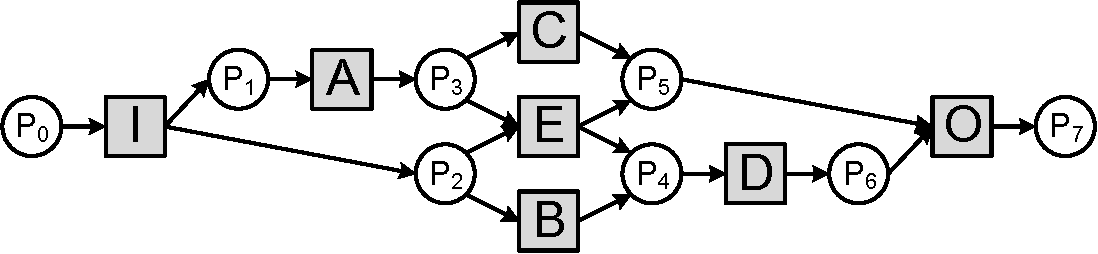
\includegraphics[width=0.9\textwidth]{multi_relation_petri}
    \caption{含有多关系变迁对的WF-net}
    \label{fig:multi_relation_petri}
  \end{subfigure}
  \begin{subfigure}{1\textwidth}
    \vspace{1em}
    \centering
    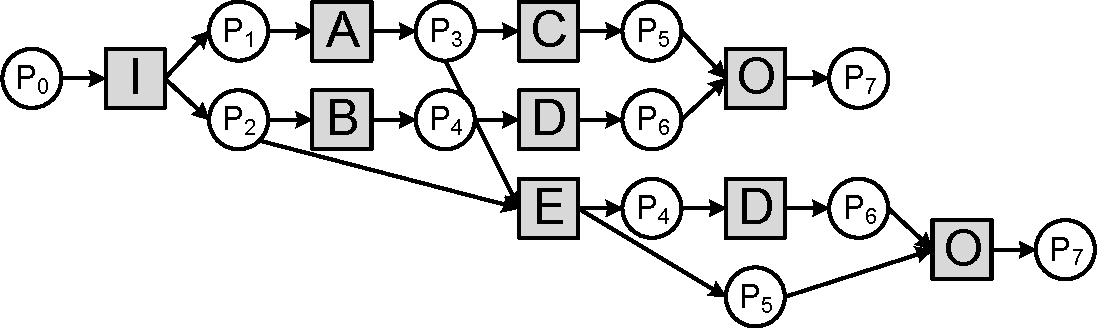
\includegraphics[width=0.9\textwidth]{multi_relation_cpu}
    \caption{图\subref{fig:multi_relation_petri}中WF-net对应的CPU}
    \label{fig:multi_relation_cpu}
  \end{subfigure}
  \vspace{6pt}
  \caption{含有多关系变迁对的模型示例}
  \label{fig:multi_relation}
\end{figure}

绝大多数算法如BP、TAR等都不能识别变迁对之间多关系的存在,因为它们将每对变迁之间的关系定义为单独一种,因此这些算法也无法准确地刻画过程模型的行为语义从而不能有效地区分含有多关系变迁对的模型。虽然RORU算法允许一对变迁之间存在多种关系,但是它并没有对一个变迁在CPU中对应多个事件的情况作处理。根据RORU的计算方法,CPU中的每个事件都被当作独立事件参与事件间RORU关系的计算,RORU并没有提及如何将多个对应事件与其他事件的关系折叠回原始变迁对之间的RORU关系。例如,在图\ref{fig:multi_relation}的模型中,RORU无法确定变迁$D$(变迁$D$在图\ref{fig:multi_relation_cpu}的CPU中有两个对应事件,变迁$O$也一样)和其他变迁之间的关系。

{\heiti 不可见变迁\qquad}不可见变迁是一类不会在过程模型执行轨迹中出现的变迁,以下情形都会导致不可见变迁的出现:
\begin{itemize}
  \item[-] 过程模型中存在只含有路由功能的无意义任务;
  \item[-] 在实际执行轨迹中会出现任务被漏记等缺失情况;
  \item[-] 过程模型中允许跳过或重做当前任务、跳回到之前某个任务的情形,但该类执行逻辑并未在过程模型的控制逻辑中表达出来。
\end{itemize}
不可见变迁不含有意义的标签,它不会在变迁执行序列中显式出现。本文使用带斜线的阴影方框表示不可见变迁。根据不可见变迁的功能,图\ref{fig:invisible_transition_types}将其分为四类。图\ref{fig:invisible_transition_skip}中的模型含有SKIP类型的不可见变迁,该类不可见变迁被用于跳过某些任务(该例中跳过了变迁$B$);图\ref{fig:invisible_transition_redo}中的模型含有REDO类型的不可见变迁,该类不可见变迁被用于重复执行某些任务(该例中重复执行变迁$B$);图\ref{fig:invisible_transition_side}中的模型含有SIDE类型的不可见变迁,该类不可见变迁与源库所或者汇库所直接相连;图\ref{fig:invisible_transition_switch}中的模型含有SWITCH类型的不可见变迁,该类不可见变迁被用于在不同分支之间切换执行权(该例中从含有变迁$A$和$C$的分支切换到含有变迁$B$和$D$的分支)。

\begin{figure}[htbp]
  \centering
  \begin{subfigure}[b]{0.48\textwidth}
    \centering
    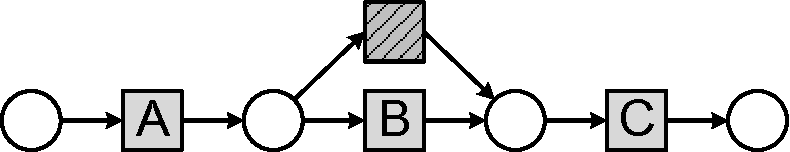
\includegraphics[width=0.98\textwidth]{invisible_transition_skip}
    \caption{SKIP类型的不可见变迁}
    \label{fig:invisible_transition_skip}
  \end{subfigure}
  \begin{subfigure}[b]{0.48\textwidth}
    \centering
    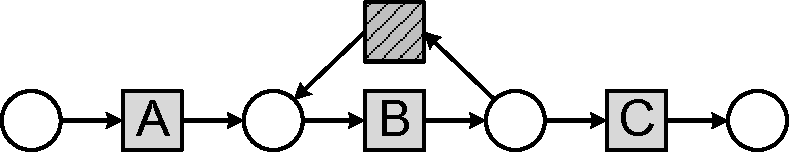
\includegraphics[width=0.98\textwidth]{invisible_transition_redo}
    \caption{REDO类型的不可见变迁}
    \label{fig:invisible_transition_redo}
  \end{subfigure}
  \begin{subfigure}[b]{0.48\textwidth}
    \vspace{1em}
    \centering
    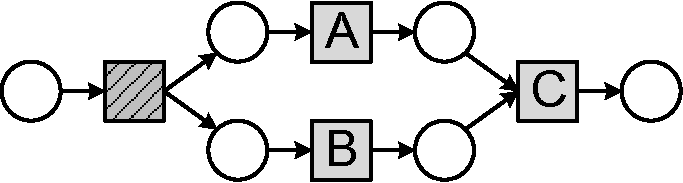
\includegraphics[width=0.98\textwidth]{invisible_transition_side}
    \caption{SIDE类型的不可见变迁}
    \label{fig:invisible_transition_side}
  \end{subfigure}
  \begin{subfigure}[b]{0.48\textwidth}
    \vspace{1em}
    \centering
    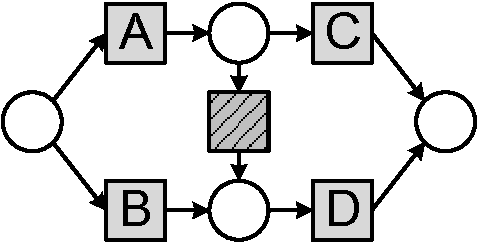
\includegraphics[width=0.7\textwidth]{invisible_transition_switch}
    \caption{SWITCH类型的不可见变迁}
    \label{fig:invisible_transition_switch}
  \end{subfigure}
  \vspace{6pt}
  \caption{四种类型的不可见变迁}
  \label{fig:invisible_transition_types}
\end{figure}

如前文所述,不可见变迁的存在能够改变过程模型的行为。图\ref{fig:sda_example}是一对含有不可见变迁的模型,两者唯一的区别在于变迁$I$和变迁$O$的关系。具体分析,在图\ref{fig:sda_example_1}的WF-net中的源库所$P_{0}$中放置一个托肯时,变迁$I$被使能,当其被触发后,会在库所$P_{1}$和库所$P_{2}$中各产生一个托肯,此时变迁$A$和变迁$B$均被使能,且满足并发执行关系;若此时将变迁$A$和变迁$B$都触发,则会在库所$P_{3}$和库所$P_{4}$中各产生一个托肯,使得中间的不可见变迁被使能;若此时只触发变迁$A$,则库所$P_{2}$和库所$P_{3}$中各有一个托肯,使得上方的不可见变迁被使能;若此时只触发变迁$B$,则库所$P_{1}$和库所$P_{4}$中各有一个托肯,使得下方的不可见变迁被使能。无论上述三种情况的哪一种发生,触发不可见变迁之后都会在库所$P_{5}$中产生一个托肯,从而使得变迁$O$被使能;当变迁$O$被触发后,过程执行完毕。该模型的变迁发生序列有四条,分别是$\langle I,A,B,O\rangle$、$\langle I,B,A,O\rangle$、$\langle I,A,O\rangle$和$\langle I,B,O\rangle$
。

与之相对应的是图\ref{fig:sda_example_2}中的WF-net,该模型中的变迁$A$和变迁$B$可以都被跳过而不被触发。当在源库所$P_{0}$中放置一个托肯时,变迁$I$被使能,当其被触发后,会在库所$P_{1}$和库所$P_{2}$中各产生一个托肯,此时变迁$A$和变迁$B$均被使能,上方和下方的两个不可见变迁也被使能了,且分别和变迁$A$、变迁$B$满足竞争关系;此时可以在上方的不可见变迁和变迁$A$中、下方的不可见变迁和变迁$B$中各选择一个触发,且触发过程满足并行关系。无论选择哪两个变迁触发,都会在库所$P_{3}$和库所$P_{4}$中各产生一个托肯,从而使得变迁$O$被使能;当变迁$O$被触发后,过程执行完毕。该模型的变迁发生序列有五条,分别是$\langle I,A,B,O\rangle$、$\langle I,B,A,O\rangle$、$\langle I,A,O\rangle$、$\langle I,B,O\rangle$和$\langle I,O\rangle$。

两个模型的行为差异在于后者比前者多了一条变迁发生序列,即变迁$I$和变迁$O$可以紧邻发生。诸如CBP、4C和RORU等以任务间关系为基础的过程模型行为语义刻画方法都没有考虑任务间紧邻关系,所以无法区分这组模型的行为语义。实际上,图\ref{fig:sda_example_1}的模型中的变迁$I$和变迁$O$满足“间接总是因果关系”,即$I\overset{\text{\tiny{IA}}}{\rightarrow}O$,而图\ref{fig:sda_example_2}的模型中的变迁$I$和变迁$O$满足“直接总是因果关系”,即$I\overset{\text{\tiny{DA}}}{\rightarrow}O$。两个模型的ExRORU关系矩阵如表\ref{tab:sda_example_matrix}所示,两个模型的行为差异主要体现在变迁$I$和变迁$O$之间的因果关系和逆因果关系上。因此,ExRORU算法可以检测该组模型之间的差异。

\begin{table}[htbp]
  \centering
  % \setlength\tabcolsep{4pt}
  \caption{图\ref{fig:sda_example}中两个模型的ExRORU矩阵}
  \label{tab:sda_example_matrix}
  \begin{subtable}{1\textwidth}
    \centering
    \caption{图\ref{fig:sda_example_1}中模型的ExRORU矩阵}
    \label{tab:sda_example_1_matrix}
    \begin{minipage}[b]{0.3\textwidth}
      \centering
      \begin{tabular}{|c|c|c|c|c|} \hline
        $\rightarrow$ & $I$ & $A$ & $B$ & $O$\\ \hline
        $I$ & $\overset{\text{\tiny{N}}}{\rightarrow}$ & $\overset{\text{\tiny{DS}}}{\rightarrow}$ & $\overset{\text{\tiny{DS}}}{\rightarrow}$ & $\overset{\text{\tiny{IA}}}{\rightarrow}$\\ \hline
        $A$ & $\overset{\text{\tiny{N}}}{\rightarrow}$ & $\overset{\text{\tiny{N}}}{\rightarrow}$ & $\overset{\text{\tiny{N}}}{\rightarrow}$ & $\overset{\text{\tiny{DA}}}{\rightarrow}$\\ \hline
        $B$ & $\overset{\text{\tiny{N}}}{\rightarrow}$ & $\overset{\text{\tiny{N}}}{\rightarrow}$ & $\overset{\text{\tiny{N}}}{\rightarrow}$ & $\overset{\text{\tiny{DA}}}{\rightarrow}$\\ \hline
        $O$ & $\overset{\text{\tiny{N}}}{\rightarrow}$ & $\overset{\text{\tiny{N}}}{\rightarrow}$ & $\overset{\text{\tiny{N}}}{\rightarrow}$ & $\overset{\text{\tiny{N}}}{\rightarrow}$\\ \hline
      \end{tabular}
    \end{minipage}
    \begin{minipage}[b]{0.3\textwidth}
      \centering
      \begin{tabular}{|c|c|c|c|c|} \hline
        $\leftarrow$ & $I$ & $A$ & $B$ & $O$\\ \hline
        $I$ & $\overset{\text{\tiny{N}}}{\leftarrow}$ & $\overset{\text{\tiny{N}}}{\leftarrow}$ & $\overset{\text{\tiny{N}}}{\leftarrow}$ & $\overset{\text{\tiny{N}}}{\leftarrow}$\\ \hline
        $A$ & $\overset{\text{\tiny{DA}}}{\leftarrow}$ & $\overset{\text{\tiny{N}}}{\leftarrow}$ & $\overset{\text{\tiny{N}}}{\leftarrow}$ & $\overset{\text{\tiny{N}}}{\leftarrow}$\\ \hline
        $B$ & $\overset{\text{\tiny{DA}}}{\leftarrow}$ & $\overset{\text{\tiny{N}}}{\leftarrow}$ & $\overset{\text{\tiny{N}}}{\leftarrow}$ & $\overset{\text{\tiny{N}}}{\leftarrow}$\\ \hline
        $O$ & $\overset{\text{\tiny{IA}}}{\leftarrow}$ & $\overset{\text{\tiny{DS}}}{\leftarrow}$ & $\overset{\text{\tiny{DS}}}{\leftarrow}$ & $\overset{\text{\tiny{N}}}{\leftarrow}$\\ \hline
      \end{tabular}
    \end{minipage}
    \begin{minipage}[b]{0.3\textwidth}
      \centering
      \begin{tabular}{|c|c|c|c|c|} \hline
        $\parallel$ & $I$ & $A$ & $B$ & $O$\\ \hline
        $I$ & $\nparallel$ & $\nparallel$ & $\nparallel$ & $\nparallel$\\ \hline
        $A$ & $\nparallel$ & $\nparallel$ & $\Uparrow$ & $\nparallel$\\ \hline
        $B$ & $\nparallel$ & $\Uparrow$ & $\nparallel$ & $\nparallel$\\ \hline
        $O$ & $\nparallel$ & $\nparallel$ & $\nparallel$ & $\nparallel$\\ \hline
      \end{tabular}
    \end{minipage}
  \end{subtable}

  \begin{subtable}{1\textwidth}
    \vspace{1em}
    \centering
    \caption{图\ref{fig:sda_example_2}中模型的ExRORU矩阵}
    \label{tab:sda_example_2_matrix}
    \begin{minipage}[b]{0.3\textwidth}
      \centering
      \begin{tabular}{|c|c|c|c|c|} \hline
        $\rightarrow$ & $I$ & $A$ & $B$ & $O$\\ \hline
        $I$ & $\overset{\text{\tiny{N}}}{\rightarrow}$ & $\overset{\text{\tiny{DS}}}{\rightarrow}$ & $\overset{\text{\tiny{DS}}}{\rightarrow}$ & $\overset{\text{\tiny{DA}}}{\rightarrow}$\\ \hline
        $A$ & $\overset{\text{\tiny{N}}}{\rightarrow}$ & $\overset{\text{\tiny{N}}}{\rightarrow}$ & $\overset{\text{\tiny{N}}}{\rightarrow}$ & $\overset{\text{\tiny{DA}}}{\rightarrow}$\\ \hline
        $B$ & $\overset{\text{\tiny{N}}}{\rightarrow}$ & $\overset{\text{\tiny{N}}}{\rightarrow}$ & $\overset{\text{\tiny{N}}}{\rightarrow}$ & $\overset{\text{\tiny{DA}}}{\rightarrow}$\\ \hline
        $O$ & $\overset{\text{\tiny{N}}}{\rightarrow}$ & $\overset{\text{\tiny{N}}}{\rightarrow}$ & $\overset{\text{\tiny{N}}}{\rightarrow}$ & $\overset{\text{\tiny{N}}}{\rightarrow}$\\ \hline
      \end{tabular}
    \end{minipage}
    \begin{minipage}[b]{0.3\textwidth}
      \centering
      \begin{tabular}{|c|c|c|c|c|} \hline
        $\leftarrow$ & $I$ & $A$ & $B$ & $O$\\ \hline
        $I$ & $\overset{\text{\tiny{N}}}{\leftarrow}$ & $\overset{\text{\tiny{N}}}{\leftarrow}$ & $\overset{\text{\tiny{N}}}{\leftarrow}$ & $\overset{\text{\tiny{N}}}{\leftarrow}$\\ \hline
        $A$ & $\overset{\text{\tiny{DA}}}{\leftarrow}$ & $\overset{\text{\tiny{N}}}{\leftarrow}$ & $\overset{\text{\tiny{N}}}{\leftarrow}$ & $\overset{\text{\tiny{N}}}{\leftarrow}$\\ \hline
        $B$ & $\overset{\text{\tiny{DA}}}{\leftarrow}$ & $\overset{\text{\tiny{N}}}{\leftarrow}$ & $\overset{\text{\tiny{N}}}{\leftarrow}$ & $\overset{\text{\tiny{N}}}{\leftarrow}$\\ \hline
        $O$ & $\overset{\text{\tiny{DA}}}{\leftarrow}$ & $\overset{\text{\tiny{DS}}}{\leftarrow}$ & $\overset{\text{\tiny{DS}}}{\leftarrow}$ & $\overset{\text{\tiny{N}}}{\leftarrow}$\\ \hline
      \end{tabular}
    \end{minipage}
    \begin{minipage}[b]{0.3\textwidth}
      \centering
      \begin{tabular}{|c|c|c|c|c|} \hline
        $\parallel$ & $I$ & $A$ & $B$ & $O$\\ \hline
        $I$ & $\nparallel$ & $\nparallel$ & $\nparallel$ & $\nparallel$\\ \hline
        $A$ & $\nparallel$ & $\nparallel$ & $\Uparrow$ & $\nparallel$\\ \hline
        $B$ & $\nparallel$ & $\Uparrow$ & $\nparallel$ & $\nparallel$\\ \hline
        $O$ & $\nparallel$ & $\nparallel$ & $\nparallel$ & $\nparallel$\\ \hline
      \end{tabular}
    \end{minipage}
  \end{subtable}
\end{table}

图\ref{fig:invisible_transition_examples}给出了更多的含有不可见变迁的过程模型对。本文的ExRORU算法可以检测到其中各组模型之间的行为差异。在图\ref{fig:invisible_transition_a}的上方模型中,变迁$A$和变迁$B$满足“直接总是因果关系”,即$A\overset{\text{\tiny{DA}}}{\rightarrow}B$,变迁$A$和变迁$C$满足“间接总是因果关系”,即$A\overset{\text{\tiny{IA}}}{\rightarrow}C$;而在下方模型中,变迁$A$和变迁$B$满足“直接有时因果关系”,即$A\overset{\text{\tiny{DS}}}{\rightarrow}B$,变迁$A$和变迁$C$满足“直接总是因果关系”,即$A\overset{\text{\tiny{DA}}}{\rightarrow}C$。

在图\ref{fig:invisible_transition_b}和图\ref{fig:invisible_transition_c}的上方模型中,变迁$B$和变迁$C$都满足“有时并行关系”,即$B\Uparrow C$,而在两幅图的下方模型中,变迁$B$和变迁$C$都满足“总是并行关系”,即$B\Updownarrow C$。

CBP等算法不考虑任务间紧邻关系也不区分并行关系的不确定性,所以无法区分图中的三组模型。TAR算法虽然考虑了任务间紧邻关系,但是对于并行关系刻画的不准确导致了它无法区分图\ref{fig:invisible_transition_b}和图\ref{fig:invisible_transition_c}中的两对模型。类似的,RORU算法无法处理这些含有不可见变迁的模型,且它不能计算图\ref{fig:invisible_transition_c}中这样带环的模型。

\begin{figure}[htbp]
  \centering
  \begin{subfigure}{1\textwidth}
    \centering
    \begin{minipage}[b]{0.45\textwidth}
      \centering
      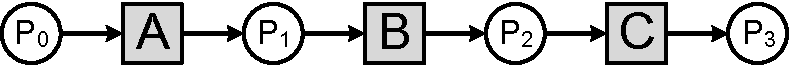
\includegraphics[width=1\textwidth]{invisible_transition_a_1}
    \end{minipage}
    \hspace{1em}
    \begin{minipage}[b]{0.45\textwidth}
      \centering
      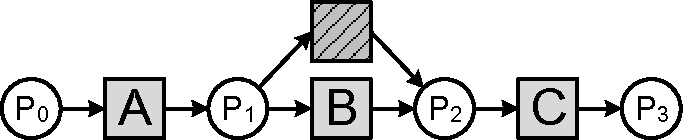
\includegraphics[width=1\textwidth]{invisible_transition_a_2}
    \end{minipage}
    \caption{}
    \label{fig:invisible_transition_a}
  \end{subfigure}
  \begin{subfigure}{1\textwidth}
    \vspace{1em}
    \centering
    \begin{minipage}[]{0.45\textwidth}
      \centering
      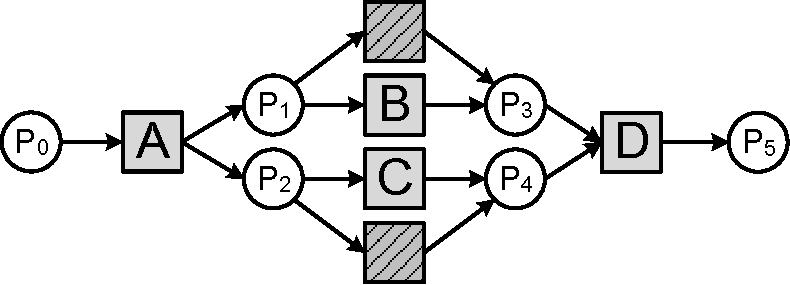
\includegraphics[width=1\textwidth]{invisible_transition_b_1}
    \end{minipage}
    \hspace{1em}
    \begin{minipage}[]{0.45\textwidth}
      \centering
      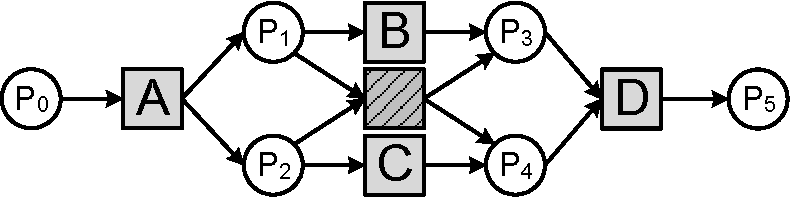
\includegraphics[width=1\textwidth]{invisible_transition_b_2}
    \end{minipage}
    \caption{}
    \label{fig:invisible_transition_b}
  \end{subfigure}
  \begin{subfigure}{1\textwidth}
    \vspace{1em}
    \centering
    \begin{minipage}[]{0.45\textwidth}
      \centering
      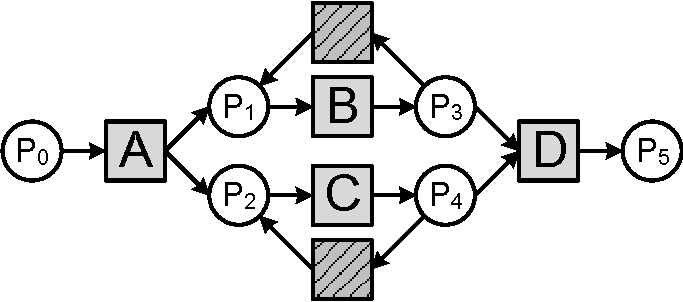
\includegraphics[width=1\textwidth]{invisible_transition_c_1}
    \end{minipage}
    \hspace{1em}
    \begin{minipage}[]{0.45\textwidth}
      \centering
      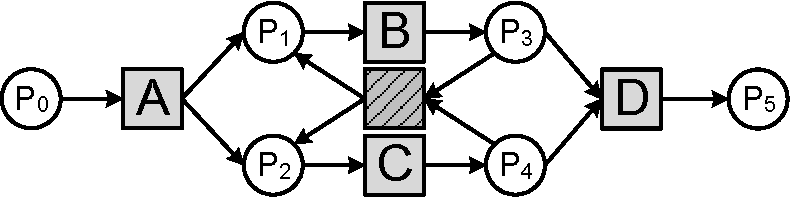
\includegraphics[width=1\textwidth]{invisible_transition_c_2}
    \end{minipage}
    \caption{}
    \label{fig:invisible_transition_c}
  \end{subfigure}
  \vspace{6pt}
  \caption{含有不可见变迁的WF-net示例}
  \label{fig:invisible_transition_examples}
\end{figure}

\subsection{性能实验}\label{subsec:efficiency}
本文使用企业中的实际模型作为数据集测试ExRORU算法的性能,表\ref{tab:efficiency_dataset}给出了这些数据集的基本结构特征。将ExRORU算法分别应用到这些数据集上,表格的最后一列是ExRORU算法在抽取每个过程模型行为特征的平均耗时。
\begin{itemize}
  \item[-] SAP数据集来自于世界著名ERP(Enterprise Resource Planning,企业资源计划)服务提供商SAP公司。原始的SAP数据集中包含604个SAP参考模型,本文删除了其中不满足定义\ref{def:sound}所述合理性的模型。最终筛选后的数据集包含389个模型。
  \item[-] DG数据集来自于东方锅炉股份有限公司,包含94个模型。东方锅炉股份有限公司是中国一流的火力发电设备、核电站设备、电机辅机、环保设备、化工容器、煤气化设备等的制造商和服务提供商。
  \item[-] TC数据集来自于唐山轨道客车有限责任公司,包含89个模型。始建于1881年的唐山轨道客车有限责任公司是中国第一家轨道装备制造企业。
\end{itemize}

从表\ref{tab:efficiency_dataset}中可以看出,ExRORU算法在来自企业的实际过程模型数据集中表现良好,能够在几毫秒至几十毫秒的时间范围内抽取过程模型的ExRORU关系矩阵,该耗时规模在实际应用中完全满足业务需求。

\begin{table}[htbp]
  \centering
  \caption{各企业实际业务过程模型集的结构特征及ExRORU算法的性能表现}
  \label{tab:efficiency_dataset}
  \begin{tabular}{lrrrrrrrr}
    \toprule[1.5pt]
    数据集 & 规模 & \tabincell{r}{平均\\变迁数} & \tabincell{r}{平均\\库所数} & \tabincell{r}{平均\\边数} & \tabincell{r}{最大\\变迁数} & \tabincell{r}{最大\\库所数} & \tabincell{r}{最大\\边数} & \tabincell{r}{平均耗时\\(毫秒)}\\ \midrule[1pt]
    SAP & 389 & 4.47 & 7.51 & 11.51 & 21 & 31 & 56 & 1.43\\
    DG & 94 & 8.56 & 8.89 & 17.78 & 34 & 33 & 70 & 10.89\\
    TC & 89 & 11.47 & 10.28 & 22.93 & 28 & 29 & 58 & 15.34\\
    \bottomrule[1.5pt]
  \end{tabular}
\end{table}

\subsection{扩展性实验}\label{subsec:scalability}
诸多过程模型行为语义刻画和相似性度量算法都会面临状态爆炸问题,即含有高并发分支的模型有巨大数量的状态,从而无法被相应算法快速处理。为了测试ExRORU在含有高并发分支的模型中的性能,本文设计了两组模型用于扩展性实验。第一组模型包含11个过程模型,依次含有$5,10,15,...,55$个并发分支,每个并发分支仅含有一个可见变迁,该组模型被用于进行宽度扩展性实验;第二组模型也包含11个过程模型,不同的是,该组中的每个模型都有5个并发分支,但分支上的变迁数依次递增,11个模型的分支上分别含有$1,2,3,...,11$个可见变迁,该组模型被用于进行深度扩展性实验。使用ExRORU算法分别抽取两组过程模型的行为特征的时间消耗如图\ref{fig:scalability}所示。

\begin{figure}[htbp]
  \centering
  \begin{subfigure}{0.48\textwidth}
    \centering
    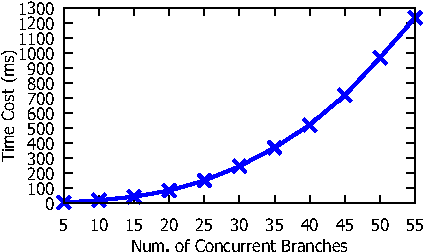
\includegraphics[width=1\textwidth]{scalability_breadth}
    \caption{宽度扩展性实验}
    \label{fig:scalability_breadth}
  \end{subfigure}
  \begin{subfigure}{0.48\textwidth}
    \centering
    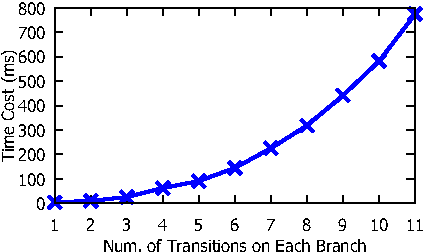
\includegraphics[width=1\textwidth]{scalability_depth}
    \caption{深度扩展性实验}
    \label{fig:scalability_depth}
  \end{subfigure}
  \vspace{6pt}
  \caption{ExRORU算法的扩展性事件结果}
  \label{fig:scalability}
\end{figure}

考虑到ExRORU算法包含任务间关系的诸多细节,扩展性实验的结果是完全可接受的。ExRORU是目前唯一可以同时处理多种复杂结构——如不可见变迁、非自由选择结构、多关系、循环结构——的算法,这显示了其杰出的性能。

\section{本章小结}
本章介绍了ExRORU算法的实现方案和实验结果。通过与其他过程模型行为语义刻画算法和相似性度量算法的比较,ExRORU拥有更为精细的刻画粒度,在含有各种复杂结构的过程模型中表现优异。同时,本文使用来自企业的实际业务过程模型数据集验证ExRORU算法的效率并使用人工创建的含高并发分支结构的过程模型数据集验证ExRORU算法的扩展性,两项实验均表明了ExRORU算法兼顾了性能和效率。